\documentclass[a4paper,11pt]{exam}
    \usepackage{hyperref}
    \ifx\pdftexversion\undefined
       \usepackage{epsfig}
    \else
       \usepackage[pdftex]{graphics}
    \fi
    \usepackage{epsfig}
    \usepackage{verbatim}
\begin{document}
    \extraheadheight{.5in}
    \firstpageheader{\large\sf CS2105}%
    {\large\sf National University of Singapore\\ School of Computing \\
    \LARGE\sf Assignment 2}%
    {\large\sf Semester 2 10/11}
    \firstpageheadrule
    \pagestyle{headandfoot}

    \section*{Deadline}

    27 March, 2011 (Sunday), 11:59pm.

    \section*{Objective}

    In this assignment, you will implement a reliable transfer protocol on top of a unreliable channel that can drop packets randomly (but always deliver in order and corruption-free).

    \section*{Pre-requisite}

You are expected to be familiar with the alternating bit protocol (rdt 3.0).

The assignment will be done under a controlled, UNIX environment. Familarity with UNIX environment (how to copy/move/delete/edit files, how to compile and run programs, etc.) is assumed.

\section*{Administrative Matters}

This is an \textit{individual} assignment.

An account has been setup for you on host cs2105-z.comp.nus.edu.sg. To access your account, ssh to the host and login using your SoC UNIX username and password \textit{from a SoC host or through SoC VPN}.

If you have any questions or encounter any problems with the steps discussed in the assignment, please contact the teaching staff through CS2105's blog.

\section*{Introduction}

For this assignment, you are given the code for a receiver and sender for three network layers: application, reliable transport (RDT), and unreliable transport (UDT).

The UDTSender and UDTReceiver classes simulate a networking layer that delivers packets unreliably.  Packet can get loss randomly.  However, for simplicity, you can assume that this layer delivers packets in order and never corrupts the packets.

The FileSender and FileReceiver classes are the application that we use for this assignment.  The FileReceiver basically is a server that waits for connection, receives a file, and saves the file onto the disk with a given name.  To run FileReceiver, use
\begin{verbatim}
  java FileReceiver <port> <filename>
\end{verbatim}
For example,
\begin{verbatim}
  java FileReceiver 9000 foo.zip
\end{verbatim}
listens on port 9000 for connection and dumps the bytes received into a file named foo.zip.

The FileSender program is basically a file uploader that connects to FileReceiver and sends the data read from a given file to FileReceiver.  To run FileSender, 
\begin{verbatim}
  java FileSender <filename> <hostname> <port>
\end{verbatim}
For example, 
\begin{verbatim}
  java FileSender foo.zip suna.comp.nus.edu.sg 9000
\end{verbatim}
connects to a FileReceiver running on suna.comp.nus.edu.sg at port 9000 and uploads foo.zip to the server.

Obviously, FileSender and FileReceiver require data delivery to be reliable (data sent cannot be lost).  This is where you come in.  

\section*{Your Tasks}

You are also provided with two classes, RDTSender and RDTReceiver, that interface between the application (FileSender and FileReceiver) and the unreliable data transport (UDTSender and UDTReceiver).  RDTSender and RSTReceiver should employ techniques from Lecture 3, including acknowledgement, retransmission, timeout, and sequence number, to make sure that data to be delivered from ``above'' is sent correctly to the other side.   You need not, however, implement windowing nor checksum.

So, your task in this assignment is to modify the given RDTSender.java and RDTReceiver.java such that FileSender and FileReceiver will work correctly -- the received file is exactly the same as the file uploaded.  

You should read the given set of source code carefully to understand the interaction between the different classes.  The code is documented and should be pretty self-explanatory.  There are only about 300 lines of code in total.

Figure 1 shows the overall relationship between the classes in this assignment.

\begin{figure}
	\begin{center}
	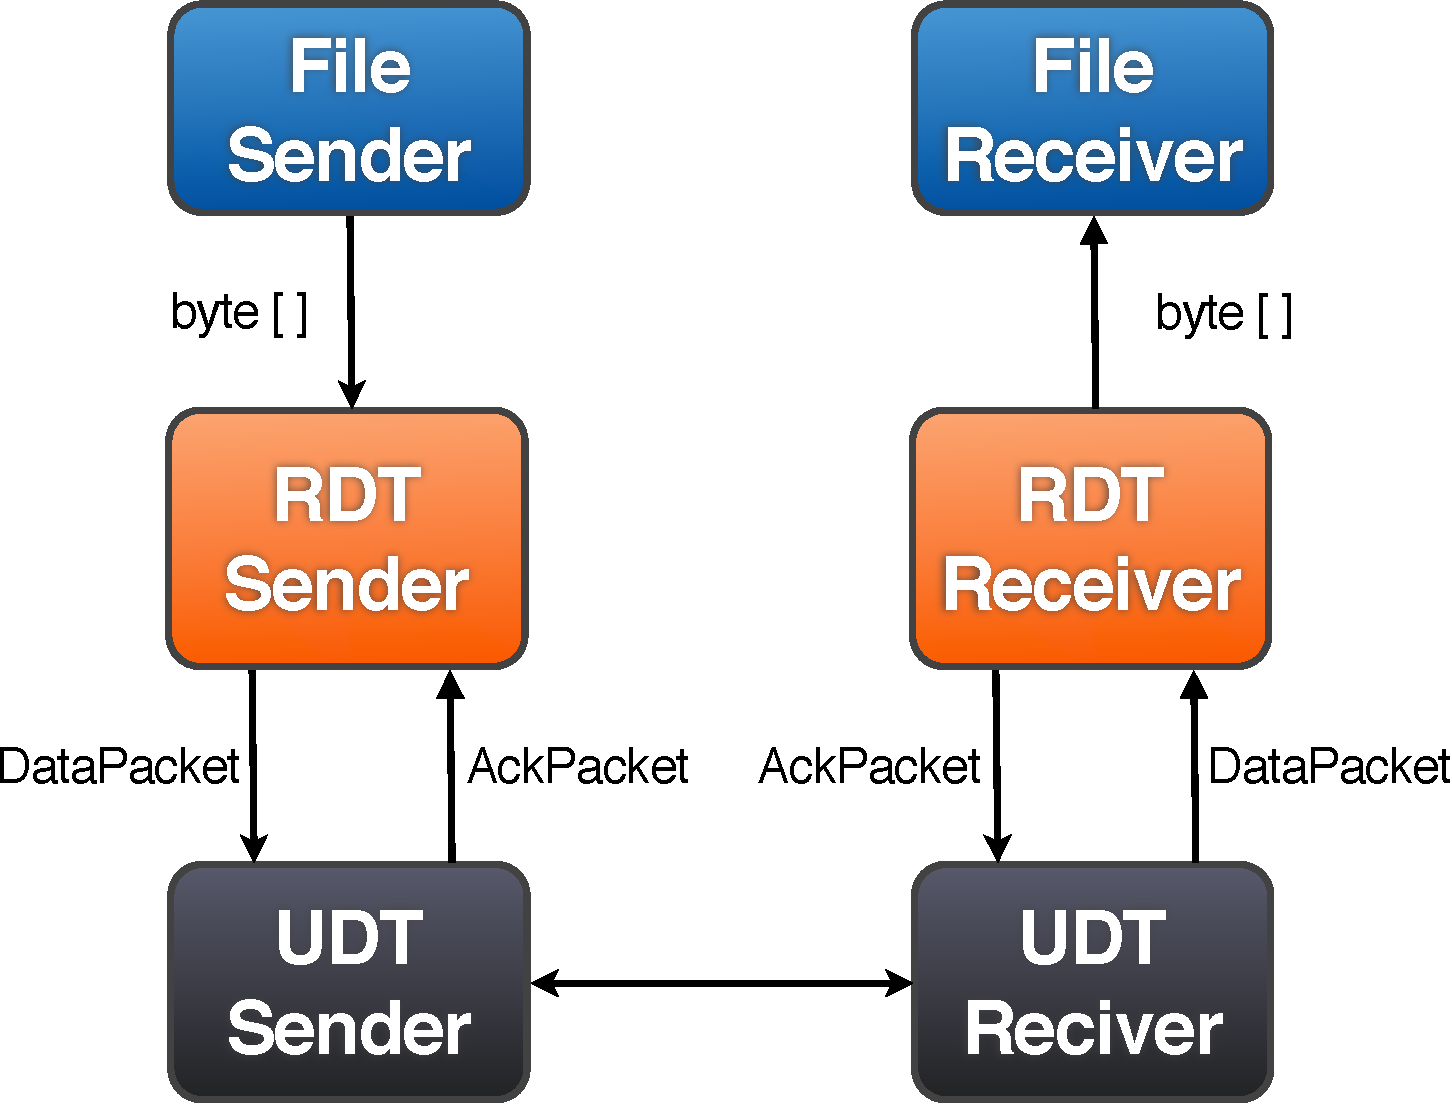
\includegraphics[scale=0.25]{flow-crop.pdf}
	\caption{Interaction between the Classes}
	\end{center}
\end{figure}

\section*{How to Do It in Java}

\subsection*{Timer}

You will need two java.util.* classes to implement timeout.  The Timer class schedules a task to be executed periodically after a certain delay, while the TimerTask class implements the code that you want to execute periodically.  For example, to print a given number after 5 seconds, and subsequently every 5 seconds, you create the following task, 
\newpage

\begin{verbatim}
class NumberPrinter extends TimerTask {
  int x;
  NumberPrinter(int toPrint) {
    x = toPrint;
  } 
  public void run() {
    System.out.println(x);
  }
}
\end{verbatim}
and schedule the timer elsewhere like this.
\begin{verbatim}
  Timer timer = new Timer();
  timer.schedule(new NumberPrinter(10), 5000, 5000);
\end{verbatim}
When you want to stop printing,
\begin{verbatim}
  timer.cancel();
\end{verbatim}

\subsection*{Sending and Receiving Packets}

(This has been done for you, so this section is for your information only)

To send and receive packets, the given code uses object serialization.  Two types of packets are defined, DataPacket and AckPacket.  They are implemented in DataPacket.java and AckPacket.java respectively.  Both classes implement the Java object serialization interface, which allows an object to be ``serialized'', i.e., to be converted into a byte stream that can be written somewhere (for instance, to disk, to a socket).  The byte stream can be read and transformed back into an object.

To send and receive data packets and ack packets, the given code wraps an object I/O stream around a socket, and calls readObject() and writeObject() to read and write DataPacket objects and AckPacket objects, effectively sending and receiving packet objects between the sender and the receiver.

\section*{Your cs2105-z Account}

An account on the server, cs2105-z.comp.nus.edu.sg, has been setup for you. From within SoC (or through SoC-VPN), ssh to cs2105-z using your SoC UNIX id and password.

Copy the files prepared for you to your home directory, by executing:

\begin{verbatim}
cp -r ~sadm/a2 .
\end{verbatim}

Note that you must put your files inside the directory \texttt{a2} directly under your home directory. 

You will be responsible for the security of your own source code. Please be careful and set the correct permission for your files. They should not be readable by anyone else except the owner (chmod 600 *.java will ensure that).

Note that you will be running your FileReceiver on the same host, and therefore must use a different port number. To prevent collision, you should avoid "nice" port numbers such as 8000 or 8080.

\section*{Submission and Grading}

There is no need to submit the program by email or IVLE workbin. We will collect your assignment from your home directory on cs2105-z.comp.nus.edu.sg when the deadline is over.

We will test your assignment automatically using a grading program. For this to work, you must not modify other java files (except RDTSender and RDTReceiver) in any signficant way (println of debugging statement is OK).  If you suspect that there is a bug in these code, please contact us by posting on the blog.  

You MUST name your java program RDTSender.java and RDTReceiver.java.  We will only compile these two files when we grade. You MUST not implement additional classes in other *.java files.

\section*{Using Another Platform}

If you like to work on your assignment on other platforms (Windows, Mac) that you are more familiar with, you are free to do so. But when you submit your assignment, you should ensure that your program runs properly under cs2105-z.comp.nus.edu.sg and your java code is located under \$HOME/a2 on cs2105-z.comp.nus.edu.sg.

\section*{Plagiarism Warning}

You are free to discuss the assignment with your peers. But, ultimately, you should write your own code. We employ zero-tolerance policy against plagiarism. If you are caught copying from other student, or let others copy your code, you will receive zero for this assignment. Further disciplinary action may be taken by the school.

\section*{Grading}

\begin{itemize}
\item 2 marks: Implement sequence number correctly.
\item 2 marks: Implement acknowledgement correctly.
\item 2 marks: Implement retransmission correctly.
\item 4 marks: Implement timeout correctly.
\end{itemize}

We will deduct one marks for every failure to following instructions (wrong directory name, wrong filename, etc.)

\vfill
\center\Huge{THE END}
\end{document}
